% Extension icon — an isometric L-tromino of three unit cubes: two plain
% hexahedra (top row) and one tetrahedralized cube (bottom-right).
% Flat teal fill, white edges — same palette and cube geometry as the
% sibling project MDPA-Preview's logo (icons/tikz-icon/icon.tex there).
% Cabinet projection (depth offset = 1/4 of the face size, shallower than a
% true cube) plus a whole-scene tilt.
%
% Only genuinely EXTERIOR faces are drawn — the mesh is opaque, not
% translucent, so a face sandwiched against a neighboring cube is skipped
% entirely rather than drawn as if visible:
%   A (top-left)            : front + top   (its right face abuts B)
%   B (top-right)            : front + top + right (no neighbors)
%   C (bottom-right, tet'd)  : front + right (its top face abuts B)
% C's tet split fans from C-fbr — the one vertex shared by both of its
% visible faces — so each diagonal lies on a real exterior face instead of
% cutting through the solid.
%
% A drafting-compass badge (opaque white contrast disc + teal legs/hinge)
% sits over the tet-meshed cube in place of MDPA-Preview's magnifier —
% CAD-Preview reads/edits B-rep CAD geometry, so the compass (the classic
% drafting tool for striking circles/arcs) is the more fitting nod than a
% "preview" magnifying glass. The needle leg plants on a point, the pencil
% leg trails a shallow crescent, evoking the tool mid-stroke.
% Rendered to images/icon.png (white bg) and images/icon_transparency.png
% (transparent) by `make icon` — see icons/README.md.
\documentclass[tikz,border=2mm]{standalone}
\usetikzlibrary{calc}
\definecolor{cadteal}{RGB}{0,128,128}
\begin{document}
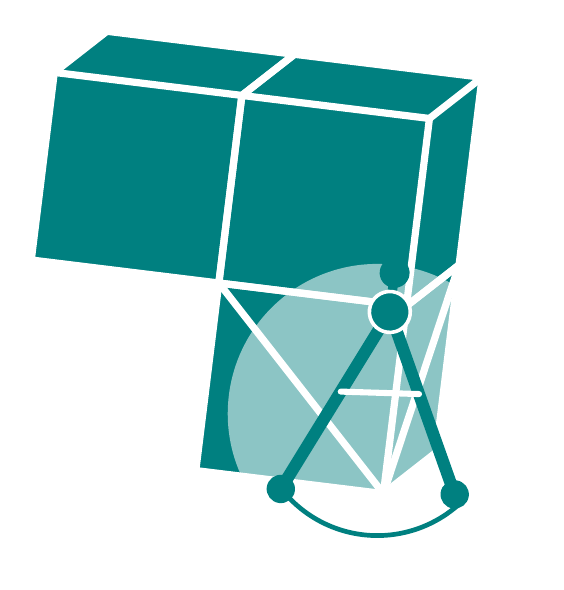
\begin{tikzpicture}[line width=2.6pt, line cap=round, line join=round, x=1mm,y=1mm, rotate=-7]
  % --- cube A (top-left) ---
  \coordinate (A-fbl) at (0,24);
  \coordinate (A-fbr) at (24,24);
  \coordinate (A-ftr) at (24,48);
  \coordinate (A-ftl) at (0,48);
  \coordinate (A-btr) at (30,54);
  \coordinate (A-btl) at (6,54);
  % --- cube B (top-right) ---
  \coordinate (B-fbl) at (24,24);
  \coordinate (B-fbr) at (48,24);
  \coordinate (B-ftr) at (48,48);
  \coordinate (B-ftl) at (24,48);
  \coordinate (B-bbr) at (54,30);
  \coordinate (B-btr) at (54,54);
  \coordinate (B-btl) at (30,54);
  % --- cube C (bottom-right, under B — the tetrahedralized cell) ---
  \coordinate (C-fbl) at (24,0);
  \coordinate (C-fbr) at (48,0);
  \coordinate (C-ftr) at (48,24);
  \coordinate (C-ftl) at (24,24);
  \coordinate (C-bbr) at (54,6);
  \coordinate (C-btr) at (54,30);

  % === fills (flat teal, faces first so edges draw crisply on top) ===
  \fill[cadteal] (A-fbl) -- (A-fbr) -- (A-ftr) -- (A-ftl) -- cycle;
  \fill[cadteal] (A-ftl) -- (A-btl) -- (A-btr) -- (A-ftr) -- cycle;

  \fill[cadteal] (B-fbl) -- (B-fbr) -- (B-ftr) -- (B-ftl) -- cycle;
  \fill[cadteal] (B-ftl) -- (B-btl) -- (B-btr) -- (B-ftr) -- cycle;
  \fill[cadteal] (B-fbr) -- (B-bbr) -- (B-btr) -- (B-ftr) -- cycle;

  \fill[cadteal] (C-fbl) -- (C-fbr) -- (C-ftr) -- (C-ftl) -- cycle;
  \fill[cadteal] (C-fbr) -- (C-bbr) -- (C-btr) -- (C-ftr) -- cycle;

  % === edges (white wireframe) ===
  \draw[white] (A-fbl) -- (A-fbr) -- (A-ftr) -- (A-ftl) -- cycle;
  \draw[white] (A-ftl) -- (A-btl) -- (A-btr) -- (A-ftr);

  \draw[white] (B-fbl) -- (B-fbr) -- (B-ftr) -- (B-ftl) -- cycle;
  \draw[white] (B-ftl) -- (B-btl) -- (B-btr) -- (B-ftr);
  \draw[white] (B-fbr) -- (B-bbr) -- (B-btr);

  \draw[white] (C-fbl) -- (C-fbr) -- (C-ftr) -- (C-ftl) -- cycle;
  \draw[white] (C-fbr) -- (C-bbr) -- (C-btr) -- (C-ftr);

  % === cube C tet split: fan from C-fbr (shared by its front & right faces) ===
  \draw[white] (C-fbr) -- (C-ftl);
  \draw[white] (C-fbr) -- (C-btr);

  % === drafting-compass badge (CAD, not "preview") — opaque white contrast
  % disc (so the compass reads clearly on both the teal mesh and the white
  % page background, same trick as MDPA's lens) + teal legs/hinge/arc ===
  \coordinate (K-c) at (46,10);
  \fill[white, fill opacity=0.55] (K-c) circle (19);

  \coordinate (K-piv) at (46,23);
  \coordinate (K-fl) at (35,-1);   % needle leg foot (the pivot of the circle it strikes)
  \coordinate (K-fr) at (57,1);    % pencil leg foot (traces the circle)

  % shallow crescent of the circle being struck, sagging just below the
  % two feet — a hint of the traced arc, not a full sweep
  \draw[cadteal, line width=1.7pt]
    ($(K-c)+(-135:15.5)$) arc (-135:-39:15.5);

  % legs
  \draw[cadteal, line width=4.4pt] (K-piv) -- (K-fl);
  \draw[cadteal, line width=4.4pt] (K-piv) -- (K-fr);

  % adjustment arm (cross-brace between the legs, partway down)
  \draw[white, line width=2.2pt]
    ($(K-piv)!0.45!(K-fl)$) -- ($(K-piv)!0.45!(K-fr)$);

  % hinge head: pivot nut + finger-grip knob above it
  \draw[cadteal, line width=3.4pt, line cap=round] (K-piv) -- ++(90:5);
  \fill[cadteal] ($(K-piv)+(90:5)$) circle (1.9);
  \fill[cadteal] (K-piv) circle (2.6);
  \draw[white, line width=1.3pt] (K-piv) circle (2.6);

  % needle tip
  \fill[cadteal] (K-fl) circle (1.8);

  % pencil tip
  \fill[cadteal] (K-fr) circle (1.8);
\end{tikzpicture}
\end{document}
